\section{Transition Dipole Moment Calculations}
\label{paper_03:sec:SI}

The intensity of a vibrational transition, \(\tilde{\nu}_{if}\), is related to the dipole moment matrix element between the two states, \(\Braket{\vec{\mu}_{if}}\)

\begin{equation}
  \label{paper_03:eq:S1}
  I \left( \tilde{\nu}_{if} \right) = \frac{8\pi^{3}N_{A}}{3hc\left( 4\pi\epsilon_{0} \right)} \tilde{\nu}_{if} \left| \vec{\mu}_{if} \right|^{2} (N_{i} - N_{f})
\end{equation}

where \(N_{A}\) is Avogadro's number, \(N_{k}\) is the number of particles in the \(k\)th state and \(\left| \vec{\mu}_{if} \right|^{2}\) is the squared norm of the transition dipole moment (TDM) integral between the two states.\textsuperscript{1} Because all values in equation~\ref{paper_03:eq:S1} are constant (at a specific temperature) vibrational intensities for particular transitions are proportional to the squared norm of the TDM vector. Thus, the central property to calculate in order to evaluate the strength of the Condon approximation is \(\Braket{\vec{\mu}_{if}}\).

We can calculate the matrix elements of the dipole moment operator in a similar fashion as the bond length matrix elements were calculated in paper 1. Before, we used the value of the bond length at each grid point as a representation of the bond length operator. Similarly, we use the \(x\), \(y\), and \(z\) components of the dipole moment at each grid point (reported by a quantum chemistry program \textemdash{} in this case, Q-Chem\textsuperscript{2} \textemdash{} as the appropriate integral over the entire charge density) as a representation of the dipole moment operator,

\begin{equation}
  \label{paper_03:eq:S2}
  \vec{\mu} = \sum_{k = 1}^{3} \mu^k \widehat{k}
\end{equation}

where \(\widehat{k}\) is the \(k^{\text{th}}\) Cartesian basis vector. The dipole moment matrix elements are, for a two dimensional grid,

\begin{equation}
  \label{paper_03:eq:S3}
  \Braket{ \vec{\mu}_{if} } = \sum_{k = 1}^{3} \sum_{l = 1}^{N} \sum_{j = 1}^{N} \psi_{jl}^{i} \mu_{jl}^{k} \widehat{k} \psi_{jl}^{f}
\end{equation}

where the \(\psi_{jl}^{n}\) are the vibrational wavefunctions for state \(n\) on grid point \((j,l)\) returned by the DVR method. We have evaluated the accuracy of this method for \ce{CO2} in two ways. First, we calculate the norm of the TDM integral for the symmetric and asymmetric stretches of \ce{CO2} in the gas phase and compare these to experiment.\textsuperscript{3} The results are shown in Table~\ref{paper_03:tab:S1}, and the accuracy is excellent.

Next, we evaluated the accuracy of this method for \ce{CO2} in solution. A previously used method for evaluating the Condon approximation for vibrational reporters in solution is to (1) optimize the vibrational subsystem of interest with DFT while freezing all other degrees of freedom, (2) calculate the harmonic vibrational frequency and intensity for the vibrational subsystem using the same DFT method, then (3) repeat this for many statistically independent snapshots of the reporter in solution.\textsuperscript{4} This process was completed for \num{25} snapshots of \ce{CO2} in IL solution for the asymmetric stretch. DVR asymmetric stretch frequencies and TDMs were also calculated for the \num{25} optimized (post step 1) snapshots. In order to facilitate comparison, the square roots of the intensities were taken. The resulting values and the TDMs were divided by their respective gas phase values. These values are plotted against each other in figure~\ref{paper_03:fig:S1}. The agreement between the two methods is excellent (\(R = 0.994\)). This new method has the advantage of being essentially computationally free to perform anytime a DVR calculation has already been done. Due to the possibility of parallelization, DVR calculations can be much more computationally inexpensive than regular vibrational frequency calculations.

\textbf{References}

(1) Carbonnière, P.; Dargelos, A.; Pouchan, C. The VCI-P Code: An Iterative Variation-Perturbation Scheme for Efficient Computations of Anharmonic Vibrational Levels and IR Intensities of Polyatomic Molecules. \emph{Theor. Chem. Acc.} \textbf{2010}, \emph{125} (3--6), 543--554.

(2) Shao, Y.; Gan, Z.; Epifanovsky, E.; Gilbert, A. T. B.; Wormit, M.; Kussmann, J.; Lange, A. W.; Behn, A.; Deng, J.; Feng, X.; et al.  Advances in Molecular Quantum Chemistry Contained in the Q-Chem 4 Program Package. \emph{Mol. Phys.} \textbf{2015}, \emph{113} (2), 184--215.

(3) Downing, H. D.; Krohn, B. J.; Hunt, R. H. Coriolis Intensity Perturbations in \(\Pi - \Sigma\) Bands of \ce{CO2}. \emph{J.  Mol. Spectrosc.} \textbf{1975}, \emph{55}, 66--80.

(4) Schmidt, J. R.; Corcelli, S. A.; Skinner, J. L. Pronounced Non-Condon Effects in the Ultrafast Infrared Spectroscopy of Water.  \emph{J. Chem. Phys.} \textbf{2005}, \emph{123} (4), 044513.

\begin{table}
  \centering
  \caption{Transition dipole moments for gas phase stretching modes of \ce{CO2}.}
  \label{paper_03:tab:S1}
  \begin{longtable}[]{@{}ccc@{}}
    \toprule
    Mode & DVR (\si{\debye}) & Experiment (\si{\debye})\textsuperscript{3}\tabularnewline
    \midrule
    \endhead
    \(\omega_{s}\) & \num{1.1e-13} & \num{0.0} \tabularnewline
    \(\omega_{a}\) & \num{3.4e-1} & \num{3.3e-1} \tabularnewline
    \bottomrule
  \end{longtable}
\end{table}

\begin{figure}
  \centering
  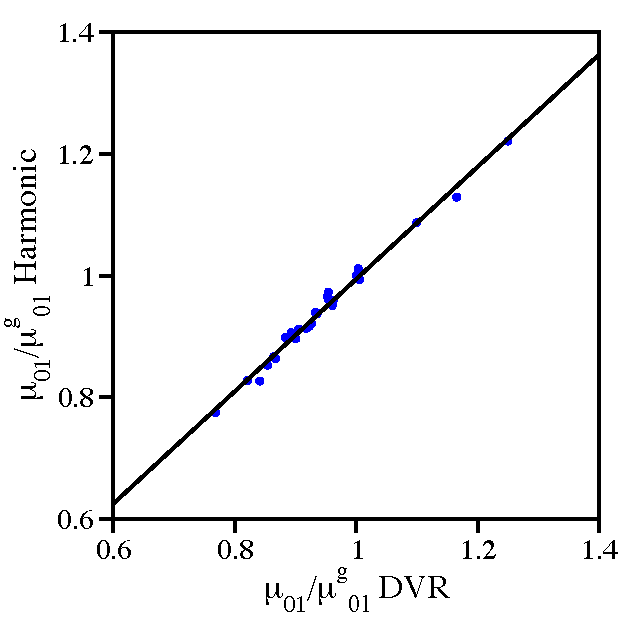
\includegraphics{figureS1.pdf}
  \caption{Normalized transition dipole moment for the asymmetric stretch of \ce{CO2} as calculated by a quantum chemistry program and as calculated by the DVR method (blue dots). The black line is the best fit line, \(y = 0.97x + 0.07\). The correlation coefficient is 0.994.}
  \label{paper_03:fig:S1}
\end{figure}
